\chapter{Metodologia}
\label{cap:metodologia}

\epigraph{\textit{"A simplicidade é o último grau de sofisticação."}}{\textbf{--- Leonardo da Vinci}}

\section{Definição dos sistemas e condições de estudo}
\label{sec:sistemas}

O presente trabalho investiga o equilíbrio líquido-líquido de sistemas ternários do tipo \{triglicerídeo + álcool + líquido iônico prótico\}, combinando três triglicerídeos, dois álcoois e dois líquidos iônicos próticos (LIPs), o que totaliza doze sistemas ternários distintos, cada um avaliado pelos dois modelos termodinâmicos (UNIFAC-LL e COSMO-SAC). Todos os sistemas são estudados a 298,15~K e pressão atmosférica.

Os triglicerídeos estudados são a trioleína (\ce{C57H104O6}), a trilinoleína (\ce{C57H98O6}) e a trilinolenina (\ce{C57H92O6}), formadas respectivamente por três cadeias de ácido oleico (uma insaturação por cadeia), ácido linoleico (duas insaturações) e ácido linolênico (três insaturações). Essa escolha permite avaliar sistematicamente o efeito do grau de insaturação da cadeia graxa sobre a miscibilidade do sistema, mantendo fixo o número de carbonos por cadeia (C18) e variando apenas o número de ligações duplas.

Os álcoois estudados são o etanol e o metanol, o que permite avaliar o efeito da cadeia alquílica do álcool (dois carbonos contra um) sobre a extensão e a posição da região bifásica, além de permitir a comparação direta com os estudos experimentais de \citeonline{trindade2019} e \citeonline{gomez2019}, que empregam metanol.

Os líquidos iônicos próticos estudados são o hexanoato de 2-hidroxietilamônio ([2-HEA][Hx]) e o hexanoato de dietilenotriamônio ([DETA][Hx]), cuja escolha se fundamenta nos resultados experimentais de \citeonline{gomez2019} e \citeonline{trindade2019}, respectivamente, que demonstraram a eficácia desses dois LIPs como cossolventes na transesterificação alcalina de óleo de soja. Os dois LIPs compartilham o mesmo ânion (hexanoato) e diferem na estrutura do cátion: o [2-HEA]$^+$ possui um grupo hidroxila na cadeia lateral e uma única carga positiva, enquanto o [DETA]$^{+3}$ apresenta uma cadeia aminada estendida, triprotonada, com maior capacidade de doação e aceitação de ligações de hidrogênio. Essa variação estrutural controlada (mesmo ânion, cátions distintos) permite isolar o efeito da estrutura do cátion sobre a miscibilidade do sistema, o que constitui um dos eixos centrais da análise comparativa proposta nos objetivos deste trabalho.

A trioleína é adotada como o sistema central de análise ao longo deste trabalho, por ser o principal triglicerídeo presente no óleo de soja, matéria-prima empregada nos estudos experimentais de referência \cite{trindade2019,gomez2019}. A utilização de triglicerídeos puros como \textit{surrogates}, em vez de um óleo vegetal real (que contém dezenas de triglicerídeos com diferentes perfis de ácidos graxos), é prática consolidada na literatura de modelagem termodinâmica de sistemas de biodiesel, pois permite representar o comportamento da fase oleosa sem a complexidade composicional de uma mistura real \cite{ferrarini2018}. A trilinoleína e a trilinolenina são incluídas como variações controladas da trioleína, isolando o efeito do grau de insaturação sobre os resultados obtidos para o sistema central.

\begin{figure}[H]
\caption{Fluxograma geral do pipeline metodológico, mostrando os dois caminhos
paralelos de cálculo do equilíbrio líquido-líquido.}
\label{fig:fluxograma_pipeline}
\centering
\resizebox{\textwidth}{!}{%
\begin{tikzpicture}[node distance=0.9cm and 1cm]

\tikzstyle{topo} = [rectangle, rounded corners, minimum width=9cm, minimum height=1cm,
    text width=8.5cm, align=center, draw=black, fill=gray!15, font=\small]
\tikzstyle{cosmo} = [rectangle, minimum width=5.5cm, minimum height=1cm,
    text width=5.2cm, align=center, draw=black, fill=teal!12, font=\small]
\tikzstyle{unifac} = [rectangle, minimum width=5.5cm, minimum height=1cm,
    text width=5.2cm, align=center, draw=black, fill=orange!12, font=\small]
\tikzstyle{merge} = [rectangle, rounded corners, minimum width=10cm, minimum height=1.1cm,
    text width=9.5cm, align=center, draw=black, fill=gray!20, font=\small]
\tikzstyle{seta} = [thick, -{Stealth[length=2mm]}]

\node (sistemas) [topo] {Sistemas ternários \{triglicerídeo + álcool + líquido iônico prótico\}: 3 triglicerídeos (trioleína, trilinoleína, trilinolenina) $\times$ 2 álcoois (etanol, metanol) $\times$ 2 LIPs ([2-HEA][Hx], [DETA][Hx]) = 12 sistemas, 298,15~K};

% coluna COSMO-SAC
\node (avogadro) [cosmo, below left=1.2cm and 2.2cm of sistemas]
    {Construção das estruturas moleculares, incluindo o par iônico neutro de cada LIP como molécula única (Avogadro)};
\node (gamess) [cosmo, below=of avogadro] {Cálculos DFT/COSMO (GAMESS)};
\node (sigmaprofiles) [cosmo, below=of gamess]
    {Geração dos $\sigma$-profiles das espécies puras, incluindo o par neutro de cada LIP};
\node (jcosmo) [cosmo, below=of sigmaprofiles]
    {JCOSMO: importação do $\sigma$-profile do par neutro como composto puro e cálculo de $\gamma_i$};
\node (ellcosmo) [cosmo, below=of jcosmo]
    {Teste de estabilidade e cálculo \textit{flash} (ELL)};

% coluna UNIFAC-LL
\node (decomp) [unifac, below right=1.2cm and 2.2cm of sistemas]
    {Decomposição em grupos funcionais UNIFAC};
\node (parametros) [unifac, below=of decomp]
    {Parâmetros de Magnussen, Rasmussen e Fredenslund (1981) e Bessa et al. (2016)};
\node (python) [unifac, below=of parametros]
    {Implementação do UNIFAC-LL em Python};
\node (ellunifac) [unifac, below=of python]
    {Teste de estabilidade e cálculo \textit{flash} (ELL)};

% nó final
\node (comparacao) [merge, below=2.0cm of $(ellcosmo)!0.5!(ellunifac)$]
    {Construção dos diagramas ternários e comparação entre os modelos: distância
    entre pontos críticos, extensão da região bifásica, coeficientes de
    distribuição $K_i$ (Capítulo 4)};

% setas
\draw [seta] (sistemas) -- (avogadro);
\draw [seta] (sistemas) -- (decomp);
\draw [seta] (avogadro) -- (gamess);
\draw [seta] (gamess) -- (sigmaprofiles);
\draw [seta] (sigmaprofiles) -- (jcosmo);
\draw [seta] (jcosmo) -- (ellcosmo);
\draw [seta] (decomp) -- (parametros);
\draw [seta] (parametros) -- (python);
\draw [seta] (python) -- (ellunifac);
\draw [seta] (ellcosmo) -- (comparacao);
\draw [seta] (ellunifac) -- (comparacao);

\end{tikzpicture}%
}
\end{figure}

Cabe uma ressalva sobre a temperatura de trabalho adotada. Os ganhos de rendimento atribuídos ao efeito cossolvente dos líquidos iônicos próticos, reportados por \citeonline{trindade2019} e \citeonline{gomez2019} e que motivam este trabalho, foram obtidos em condição reacional, a aproximadamente 60\,°C. O equilíbrio líquido-líquido modelado neste trabalho, a 298,15~K, não representa diretamente essa condição reacional, mas sim uma etapa distinta e também relevante do processo: a separação de fases do meio reacional após o resfriamento, etapa que antecede a purificação do biodiesel e que tipicamente ocorre próxima à temperatura ambiente. A cossolvência observada experimentalmente por Trindade e Gomez é, portanto, um fenômeno à temperatura de reação, enquanto os diagramas de ELL apresentados neste trabalho caracterizam o comportamento de fases numa condição posterior e distinta, ainda que igualmente relevante para o desempenho global do processo. Essa distinção é retomada na interpretação dos resultados (Seção~\ref{subsec:salting_in_out}), e a extensão dos resultados aqui apresentados para a condição reacional a 60\,°C permanece como uma limitação de escopo deste trabalho, não coberta pelos sistemas modelados.

\section{Dados experimentais para validação}
\label{sec:dados_validacao}

A avaliação da capacidade preditiva de um modelo termodinâmico requer a comparação entre os resultados simulados e dados experimentais de equilíbrio de fases. No caso do presente trabalho, essa comparação enfrenta uma limitação importante: a revisão bibliográfica conduzida não identificou dados experimentais publicados de equilíbrio líquido-líquido (composições das fases coexistentes, linhas de amarração) para os doze sistemas ternários \{triglicerídeo + álcool + líquido iônico prótico\} estudados neste trabalho. Os trabalhos de \citeonline{trindade2019} e \citeonline{gomez2019}, que constituem a motivação experimental deste estudo, reportam dados de rendimento mássico de biodiesel em função da concentração de cossolvente, mas não incluem a determinação das composições das fases em equilíbrio no sistema ternário.

Diante dessa limitação, a estratégia de validação adotada neste trabalho é dividida em duas etapas. A primeira consiste na validação metodológica do modelo COSMO-SAC em sistemas ternários análogos para os quais dados experimentais de ELL estão disponíveis na literatura.
\citeonline{xu2022} publicaram dados de ELL para sistemas do tipo \{éster + álcool + LI de imidazólio\} a 298,15 K, incluindo linhas de amarração e curvas binodais. Esses sistemas compartilham com os sistemas-alvo a presença simultânea de um éster, um álcool e um líquido iônico, o que os torna representativos para avaliar se o COSMO-SAC captura adequadamente as interações intermoleculares relevantes nessa classe de misturas. \citeonline{dominguez2014} fornecem dados de ELL para sistemas \{hidrocarboneto alifático + hidrocarboneto aromático + LI de imidazólio\} a 298,15 K, que permitem avaliar o desempenho do modelo na descrição de sistemas com líquidos iônicos em geral. Esses dois conjuntos de dados foram identificados como sistemas de referência adequados para essa validação externa; sua aplicação efetiva, contudo, limitou-se neste trabalho a uma verificação qualitativa da qualidade geométrica dos perfis sigma envolvidos (Seção~\ref{subsec:parametros_perfis}), sem uma quantificação por RMSD equivalente à realizada para o UNIFAC-LL. Essa lacuna é registrada como limitação na Seção~\ref{subsec:sintese} e na Conclusão, e sua resolução é sugerida como direção de trabalho futuro.

A segunda etapa consiste na análise dos diagramas ternários simulados para os próprios sistemas-alvo, na ausência de dados experimentais diretos. Nesse caso, a avaliação é de natureza qualitativa e apoia-se na comparação entre o comportamento previsto pelos modelos e as observações experimentais indiretas reportadas por \citeonline{trindade2019} e \citeonline{gomez2019}. Examina-se, para cada sistema, em que sentido a adição do líquido iônico prótico altera a extensão da região bifásica, e confronta-se o resultado com os ganhos de rendimento relatados por esses autores, atentando para as diferenças de temperatura, de faixa de concentração e de natureza da grandeza medida que separam as duas situações. A comparação entre os dois líquidos iônicos ([2-HEA][Hx] e [DETA][Hx]) é conduzida da mesma forma, sem que se assuma, de antemão, qual direção o resultado computacional deve tomar.

Para a validação da implementação do UNIFAC-LL, descrita na Seção \ref{sec:unifac_implementacao}, emprega-se o sistema ternário \{n-hexano + etanol + água\}, para o qual dados experimentais de ELL estão amplamente disponíveis na literatura e a parametrização de \citeonline{magnussen1981} é completa. Esse sistema serve exclusivamente como verificação da corretude da implementação computacional, e não como avaliação da capacidade do UNIFAC-LL de descrever sistemas contendo líquidos iônicos.

\section{Construção das estruturas moleculares}
\label{sec:estruturas}

As estruturas moleculares tridimensionais das nove espécies neutras envolvidas nos cálculos COSMO foram construídas no \textit{software} Avogadro (\textit{open-source}), um editor molecular que permite a construção, visualização e edição de geometrias moleculares em três dimensões \cite{avogadro2012}. As espécies modeladas são: etanol (\ce{C2H6O}), metanol (\ce{CH4O}), trioleína (\ce{C57H104O6}), trilinoleína (\ce{C57H98O6}), trilinolenina (\ce{C57H92O6}), ácido oleico (\ce{C18H34O2}), ácido linoleico (\ce{C18H32O2}) e os pares iônicos neutros [2-HEA][Hx] e [DETA][Hx]. Dessas nove, apenas os dois pares iônicos neutros foram efetivamente submetidos a cálculo DFT/COSMO no GAMESS pela autora deste trabalho (Seção~\ref{sec:dft_cosmo}); as demais sete espécies, construídas no Avogadro como parte da modelagem inicial do sistema, tiveram seus $\sigma$-profiles finais obtidos diretamente do banco de dados interno do JCOSMO (Tabela~\ref{tab:cosmo_detalhes}), já calculados e validados pelo desenvolvedor da ferramenta, de modo que a construção dessas sete no Avogadro serviu à modelagem preliminar e à conferência estrutural, mas não alimentou diretamente nenhum cálculo de química quântica realizado neste trabalho.

Para os três triglicerídeos, a geometria inicial foi obtida a partir do banco de dados interno do Avogadro, que fornece estruturas pré-construídas para diversas moléculas de interesse. Os três compartilham o mesmo núcleo de glicerol esterificado a três cadeias de ácido graxo C18, diferindo apenas no grau de insaturação de cada cadeia (uma, duas e três ligações duplas, respectivamente, para trioleína, trilinoleína e trilinolenina). A trioleína constitui o principal componente do óleo de soja, matéria-prima empregada nos estudos experimentais de referência \cite{trindade2019,gomez2019}, e é adotada como sistema central de análise (Seção~\ref{sec:sistemas}). Cada triglicerídeo possui em torno de 160 a 170 átomos, o que os torna significativamente maiores do que as demais espécies do sistema.

Os ácidos oleico e linoleico, empregados na avaliação dos sistemas com ácido graxo livre (Seção~\ref{subsec:casos_sem_separacao}), tiveram suas geometrias iniciais obtidas da mesma forma, a partir do banco de dados interno do Avogadro, e compartilham com a trioleína e a trilinoleína, respectivamente, a mesma cadeia graxa C18 com o mesmo grau de insaturação, diferindo apenas pela ausência do núcleo de glicerol e das demais duas cadeias esterificadas.

Para os líquidos iônicos próticos, conforme a estratégia de par iônico neutro adotada (Seção~\ref{sec:cosmo_li}), o cátion e o ânion de cada LIP foram construídos no Avogadro e, em seguida, efetivamente otimizados por cálculo quântico no GAMESS, integrado ao cálculo COSMO, sem etapa prévia de pré-otimização por campo de forças, como uma única molécula neutra, e não como espécies carregadas independentes. O par [2-HEA][Hx] foi montado unindo o cátion 2-hidroxietilamônio (produto da protonação da monoetanolamina, com um grupo amônio \ce{-NH3+} e um grupo hidroxila \ce{-OH} na cadeia lateral) ao ânion hexanoato, por meio de uma ligação iônica N-H$\cdots$O entre o hidrogênio ácido do grupo amônio e um dos oxigênios do carboxilato. O par [DETA][Hx] foi montado de forma análoga, unindo o cátion dietilenotriamônio triprotonado (produto da triprotonação da dietilenotriamina, com três átomos de nitrogênio protonados na cadeia) a três ânions hexanoato, um para cada sítio protonado, na estequiometria 1:3 confirmada experimentalmente por \citeonline{trindade2019}, que reporta a síntese do [DETA][Hx] a partir de 1 mol de dietilenotriamina e 3 mol de ácido hexanoico. As geometrias dos dois pares foram ajustadas manualmente no Avogadro antes de serem submetidas à otimização por cálculo quântico. Uma tentativa inicial de geração dos $\sigma$-profiles dos pares iônicos via NWChem, com compatibilização para a parametrização TURBOMOLE do JCOSMO, foi descartada após produzir cavidades moleculares com dimensões fisicamente inconsistentes (Seção~\ref{sec:jcosmo}), o que motivou a adoção exclusiva do GAMESS como pacote de química quântica para os cálculos realizados neste trabalho. Após a otimização, a integridade estrutural de cada par foi verificada pela simetria das ligações C-O do grupo carboxilato do ânion hexanoato: no par [2-HEA][Hx], as duas ligações C-O apresentaram comprimentos de 1,2682 Å e 1,2703 Å; no par [DETA][Hx], os três grupos carboxilato (um para cada sítio protonado do cátion triprotonado) apresentaram comprimentos de 1,2620/1,2692 Å, 1,2737/1,2668 Å e 1,2795/1,2693 Å, respectivamente. Em todos os casos, a diferença entre as duas ligações C-O de um mesmo carboxilato não ultrapassou 0,01 Å, padrão consistente com um carboxilato simétrico e deslocalizado. Uma perda de próton mal distribuída durante a triprotonação do DETA, com reversão a um ácido carboxílico protonado em algum dos três sítios, produziria uma assimetria muito mais acentuada entre as duas ligações C-O do carboxilato correspondente (aproximadamente 1,21 Å para a ligação C=O e 1,34 Å para a ligação C-OH), o que não foi observado em nenhum dos três sítios do [DETA][Hx].

\begin{figure}[H]
\caption{Estruturas moleculares otimizadas no Avogadro: (a) par iônico neutro [2-HEA][Hx]; (b) par iônico neutro [DETA][Hx].}
\label{fig:modelos3d}
\centering
\begin{tabular}{cc}
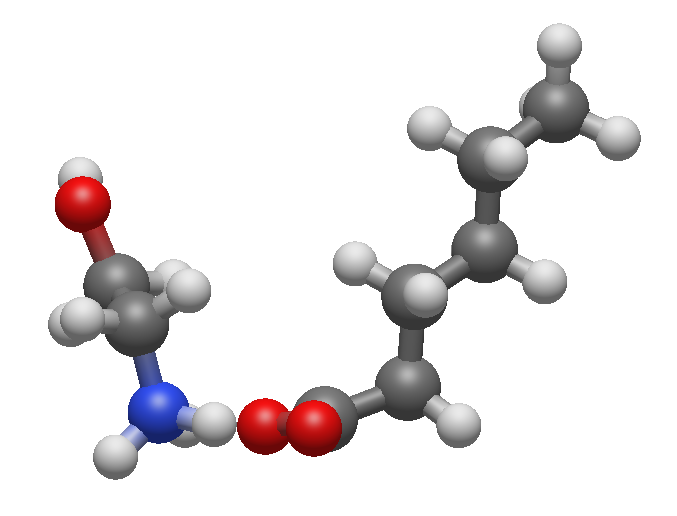
\includegraphics[width=0.42\textwidth]{imagens/2HEAHx_avogadro.png} &
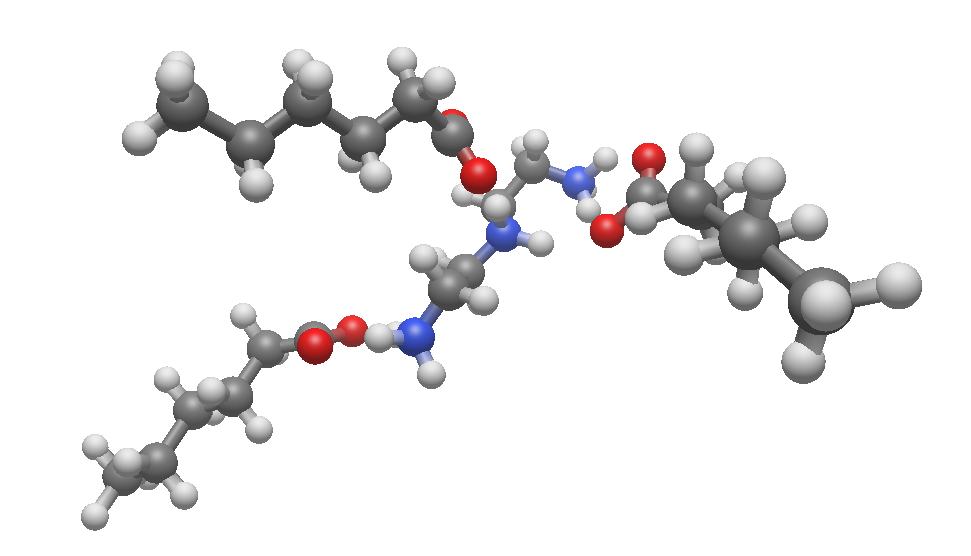
\includegraphics[width=0.42\textwidth]{imagens/DETAHx_avogadro.png} \\
(a) [2-HEA][Hx] & (b) [DETA][Hx] \\
\end{tabular}
\end{figure}

\begin{table}[H]
\caption{Propriedades físicas e estruturais das espécies envolvidas nos sistemas estudados.}
\label{tab:propriedades_especies}
\centering
\begin{tabularx}{\textwidth}{Xccc}
\toprule
\textbf{Composto} & \textbf{Abreviação} & \textbf{Fórmula molecular} & \textbf{Massa molar (g/mol)} \\
\midrule
Trioleína & --- & C\textsubscript{57}H\textsubscript{104}O\textsubscript{6} & 885,4 \\
Trilinoleína & --- & C\textsubscript{57}H\textsubscript{98}O\textsubscript{6} & 879,4 \\
Trilinolenina & --- & C\textsubscript{57}H\textsubscript{92}O\textsubscript{6} & 873,3 \\
Ácido oleico & --- & C\textsubscript{18}H\textsubscript{34}O\textsubscript{2} & 282,5 \\
Ácido linoleico & --- & C\textsubscript{18}H\textsubscript{32}O\textsubscript{2} & 280,4 \\
Etanol & --- & C\textsubscript{2}H\textsubscript{6}O & 46,1 \\
Metanol & --- & CH\textsubscript{4}O & 32,0 \\
Hexanoato de 2-hidroxietilamônio & [2-HEA][Hx] & C\textsubscript{8}H\textsubscript{19}NO\textsubscript{3} & 177,2 \\
Hexanoato de dietilenotriamônio & [DETA][Hx] & C\textsubscript{22}H\textsubscript{49}N\textsubscript{3}O\textsubscript{6} & 451,6 \\
\bottomrule
\end{tabularx}
\end{table}

\section{Cálculos DFT/COSMO e origem dos \texorpdfstring{$\sigma$}{sigma}-profiles}
\label{sec:dft_cosmo}

A qualidade das predições do modelo COSMO-SAC depende da consistência entre o nível de teoria empregado na geração dos $\sigma$-profiles e a parametrização adotada no cálculo dos coeficientes de atividade (Seção \ref{subsec:cosmo_parametros}). Neste trabalho, todos os $\sigma$-profiles utilizados são compatíveis com a parametrização GAMESS implementada no JCOSMO, conforme documentado por \citeonline{wang2009}.

Para o etanol, o metanol, a trioleína, a trilinoleína e a trilinolenina, os $\sigma$-profiles foram obtidos diretamente da base de dados interna do JCOSMO, que contém perfis pré-calculados para um conjunto extenso de compostos orgânicos convencionais \cite{mullins2006}. Os cálculos originais dessa base foram realizados no pacote GAMESS \cite{gamess2020} com o nível de teoria e os parâmetros de cavidade descritos por \citeonline{wang2009}, o que garante a consistência com a parametrização do modelo.

Para os pares iônicos neutros [2-HEA][Hx] e [DETA][Hx], que não constam na base interna do JCOSMO, os $\sigma$-profiles foram gerados por cálculos DFT/COSMO realizados no pacote GAMESS \cite{gamess2020}, seguindo o procedimento descrito por \citeonline{wang2009} para garantir a compatibilidade com a parametrização do modelo. Cada par foi calculado como uma única molécula neutra (carga total 0), conforme a estratégia de par iônico neutro adotada neste trabalho (Seção \ref{sec:cosmo_li}), e não como cátion e ânion isolados. A otimização de geometria e a determinação das cargas de blindagem no contínuo dielétrico foram realizadas de forma simultânea e autoconsistente, conforme descrito na Seção \ref{sec:cosmo_solvatacao}. Os arquivos de saída no formato \texttt{.gout} gerados pelo GAMESS foram importados diretamente no JCOSMO como compostos personalizados.

A Tabela \ref{tab:cosmo_detalhes} resume a origem dos
$\sigma$-profiles de cada espécie.

\begin{table}[H]
    \centering
    \caption{Origem dos $\sigma$-profiles utilizados nos cálculos COSMO-SAC (parametrização GAMESS no JCOSMO).}
    \label{tab:cosmo_detalhes}
    \begin{tabular}{lccc}
        \toprule
        \textbf{Espécie} & \textbf{Carga} &
        \textbf{N$^{\circ}$ de átomos} & \textbf{Origem} \\
        \midrule
        Etanol             &  0 &   9 & Base interna do JCOSMO \\
        Metanol            &  0 &   6 & Base interna do JCOSMO \\
        Trioleína          &  0 & 167 & Base interna do JCOSMO \\
        Trilinoleína       &  0 & 161 & Base interna do JCOSMO \\
        Trilinolenina      &  0 & 155 & Base interna do JCOSMO \\
        Ácido oleico       &  0 &  54 & Base interna do JCOSMO \\
        Ácido linoleico    &  0 &  52 & Base interna do JCOSMO \\
        {[2-HEA][Hx]} (par neutro) &  0 &  31 & Calculado no GAMESS \\
        {[DETA][Hx]} (par neutro)  &  0 &  80 & Calculado no GAMESS \\
        \bottomrule
    \end{tabular}
\end{table}

A geração da tabela de segmentos de superfície (área e carga de blindagem por segmento), necessária para a construção do $\sigma$-profile de cada par iônico neutro, exigiu uma modificação prévia no código-fonte do GAMESS. Na compilação padrão do pacote, essa tabela não é impressa no arquivo de saída, independentemente das palavras-chave de entrada utilizadas. A solução, documentada no repositório do Laboratório Virtual de Predição de Propriedades (LVPP)\footnote{Disponível em: \url{https://github.com/lvpp/sigma}.}, mesmo banco de dados de $\sigma$-profiles do qual o JCOSMO se utiliza, consiste em um patch aplicado ao arquivo-fonte \texttt{cosprt.src} antes da compilação, responsável pela rotina de impressão dos dados COSMO. Após a aplicação desse patch e a recompilação do GAMESS, a tabela de segmentos passou a ser impressa automaticamente, tornando desnecessária (e, em combinação com a base \texttt{d2tzvp} empregada, incompatível) a palavra-chave de entrada \texttt{COSWRT=.TRUE.}, que foi removida do arquivo de configuração dos cálculos.

A escolha de utilizar a base interna do JCOSMO para o etanol, o metanol, a trioleína, a trilinoleína e a trilinolenina, em vez de realizar novos cálculos, assegura que os $\sigma$-profiles dessas espécies são exatamente aqueles para os quais os parâmetros universais do modelo foram calibrados, evitando inconsistências que poderiam comprometer a qualidade das predições. Para os pares neutros dos LIPs, por não estarem disponíveis em nenhuma base pré-existente, o cálculo no GAMESS com o mesmo nível de teoria da base é a única forma de garantir essa consistência.

\section{Geração dos \texorpdfstring{$\sigma$}{sigma}-profiles e cálculo do ELL no JCOSMO}
\label{sec:jcosmo}

O cálculo dos coeficientes de atividade pelo modelo COSMO-SAC e a determinação do equilíbrio líquido-líquido foram realizados no \textit{software} JCOSMO, desenvolvido pelo Laboratório Virtual de Predição de Propriedades (LVPP) da Universidade Federal do Rio Grande do Sul (UFRGS) \cite{gerber2010}. O JCOSMO é uma implementação de código aberto, em linguagem Java, dos modelos COSMO-SAC e suas variantes, que permite a importação de $\sigma$-profiles a partir de diferentes pacotes de química quântica (GAMESS, TURBOMOLE, DMol3, MOPAC), o cálculo de coeficientes de atividade, testes de estabilidade de fases e a construção de diagramas de equilíbrio de fases para sistemas multicomponentes.

A execução da interface gráfica do JCOSMO em versões recentes do Java (Java 21) exigiu um ajuste na linha de comando de inicialização. A biblioteca de serialização empregada internamente pelo JCOSMO (XStream) tenta acessar, por reflexão, classes internas de módulos do Java que passaram a ser encapsulados por padrão a partir do sistema de módulos introduzido nas versões mais recentes da plataforma, o que resulta em uma exceção (\texttt{InaccessibleObjectException}) e impede a abertura do programa. A solução consiste em iniciar o JCOSMO explicitando um conjunto de flags \texttt{--add-opens}, que reabrem manualmente os pacotes necessários (dos módulos \texttt{java.base} e \texttt{java.desktop}) para acesso por reflexão, por exemplo:

\begin{verbatim}
java --add-opens java.base/java.lang=ALL-UNNAMED \
     --add-opens java.base/java.util=ALL-UNNAMED \
     --add-opens java.desktop/java.awt=ALL-UNNAMED \
     --add-opens java.desktop/javax.swing=ALL-UNNAMED \
     -jar jcosmo.jar
\end{verbatim}
% -----------------------------------------------------------------
% Escolha da variante do modelo
% -----------------------------------------------------------------

O JCOSMO disponibiliza diferentes parametrizações do COSMO-SAC, associadas aos diferentes níveis de teoria utilizados na geração dos $\sigma$-profiles. Neste trabalho, adotou-se a parametrização correspondente ao modelo GAMESS, que utiliza $\sigma$-profiles gerados com o pacote GAMESS conforme descrito por \citeonline{wang2009}. A escolha dessa parametrização foi motivada por testes preliminares nos quais uma rota alternativa (cálculos em NWChem, cujos $\sigma$-profiles seriam posteriormente compatibilizados com a parametrização TURBOMOLE do JCOSMO) produziu resultados fisicamente inconsistentes para o sistema em estudo: as cavidades moleculares geradas apresentaram dimensões significativamente superiores às esperadas (da ordem de quatro vezes a área esperada para a trioleína), resultando em $\sigma$-profiles excessivamente suavizados e em predições de afinidade trioleína-etanol incompatíveis com o comportamento experimental conhecido (miscibilidade parcial). Essa rota foi descartada, e os cálculos dos pares iônicos neutros deste trabalho foram refeitos diretamente no GAMESS (Seção~\ref{sec:dft_cosmo}), que produziu $\sigma$-profiles com distribuições de carga fisicamente coerentes; para as demais sete espécies, disponíveis na base de dados interna do JCOSMO, essa questão não se colocou, já que seus $\sigma$-profiles já haviam sido calculados e validados previamente pelo desenvolvedor da ferramenta.


% -----------------------------------------------------------------
% Incorporação dos σ-profiles dos LIPs
% -----------------------------------------------------------------

A base de dados interna do JCOSMO para o modelo GAMESS contém $\sigma$-profiles pré-calculados para um conjunto extenso de compostos orgânicos convencionais \cite{mullins2006}, incluindo os sete compostos moleculares deste trabalho (etanol, metanol, trioleína, trilinoleína, trilinolenina, ácido oleico e ácido linoleico). Os pares iônicos neutros [2-HEA][Hx] e [DETA][Hx], contudo, não constam dessa base, o que exigiu a incorporação dos $\sigma$-profiles gerados pelos cálculos DFT/COSMO realizados diretamente no GAMESS (Seção~\ref{sec:dft_cosmo}). Os arquivos \texttt{.gout} resultantes desses cálculos foram importados no JCOSMO como compostos personalizados, seguindo o mesmo procedimento de importação empregado para qualquer molécula neutra.

Uma vez que os $\sigma$-profiles de todas as nove espécies estavam disponíveis no JCOSMO, a configuração dos sistemas ternários foi feita diretamente na aba \textit{Mixture} do programa, inserindo cada líquido iônico prótico como um composto puro regular (o par neutro [2-HEA][Hx] ou [DETA][Hx]), na mesma condição dos demais componentes do sistema (triglicerídeo e álcool). Essa abordagem dispensa qualquer funcionalidade de combinação de íons separados, já que o par neutro já constitui, por si só, a unidade química completa cujo $\sigma$-profile foi previamente calculado e importado. O próprio JCOSMO normaliza internamente as frações molares informadas para cada componente da mistura, de modo que a composição do sistema ternário é definida diretamente pelas frações molares dos três compostos puros (triglicerídeo, álcool e par iônico neutro), sem etapas intermediárias de conversão.

% -----------------------------------------------------------------
% Cálculo do ELL
% -----------------------------------------------------------------

O JCOSMO é empregado exclusivamente para o cálculo dos coeficientes de atividade $\gamma_i$ de cada componente, a partir dos $\sigma$-profiles importados e da composição da mistura definida na aba \textit{Mixture}. O programa não realiza nativamente a construção de diagramas de equilíbrio de fases, de modo que o teste de estabilidade, o cálculo \textit{flash} líquido-líquido e a construção do diagrama ternário são realizados externamente, nos mesmos módulos Python desenvolvidos para o UNIFAC-LL (Seção \ref{sec:unifac_implementacao}), adaptados para consumir os coeficientes de atividade calculados pelo JCOSMO em vez dos calculados internamente pela rotina UNIFAC-LL. A comunicação entre o JCOSMO (em Java) e os módulos de estabilidade e flash (em Python) é feita por meio da biblioteca py4j, que expõe os métodos de cálculo de $\gamma_i$ do JCOSMO como uma ponte acessível diretamente do código Python.

O procedimento de cálculo do equilíbrio líquido-líquido, executado nesses módulos Python, compreende três etapas. A primeira é o teste de estabilidade de fases (critério TPD, Seção \ref{sec:ell_fundamentos}), que verifica, para uma dada composição global, se a mistura é estável como fase única ou se existe uma configuração de duas fases com energia de Gibbs total inferior. A segunda etapa é o cálculo \textit{flash} líquido-líquido, que determina as composições e as quantidades relativas das duas fases em equilíbrio a partir da composição global, resolvendo iterativamente a condição de isoatividade (Equação \ref{eq:isoatividade}) para todos os componentes do sistema. A terceira etapa é a construção do diagrama ternário, na qual o procedimento de teste de estabilidade e cálculo flash é repetido sistematicamente para uma malha de composições globais que cobre o interior do triângulo ternário, permitindo traçar a curva binodal e as linhas de amarração.

Todos os cálculos de ELL foram realizados a 298,15 K e pressão atmosférica, condições consistentes com os dados experimentais de validação (Seção \ref{sec:dados_validacao}) e com as condições empregadas nos estudos experimentais de referência \cite{trindade2019,gomez2019}.

\section{Implementação do UNIFAC-LL}
\label{sec:unifac_implementacao}

Toda a ferramenta computacional empregada neste trabalho para o cálculo do equilíbrio líquido-líquido e para a construção dos diagramas ternários foi desenvolvida pela autora, em linguagem Python, sem recurso a bibliotecas termodinâmicas prontas para essas finalidades. O conjunto é organizado em módulos com funções específicas: o cálculo dos coeficientes de atividade pelo UNIFAC-LL (contribuições combinatorial e residual), o teste de estabilidade de fases, o cálculo \textit{flash} líquido-líquido, a localização do ponto crítico, a renderização dos diagramas ternários, a interface gráfica de seleção de sistemas e o executor de fila que processa múltiplos sistemas em sequência. Empregaram-se apenas bibliotecas de uso geral (NumPy para álgebra numérica, Matplotlib para renderização e py4j para a comunicação com o JCOSMO), de modo que a formulação termodinâmica, os algoritmos de equilíbrio e a construção geométrica dos diagramas são de implementação própria.
 
Essa autoria tem uma implicação metodológica direta: como nenhuma etapa do cálculo é herdada de implementação de terceiros já validada, tornou-se necessário verificar a corretude do próprio motor de cálculo antes de aplicá-lo aos sistemas de interesse, o que é feito em duas etapas independentes descritas na Seção~\ref{sec:validacao_computacional}. A única exceção é o cálculo dos coeficientes de atividade pelo COSMO-SAC, delegado ao JCOSMO (Seção~\ref{sec:jcosmo}); todas as demais etapas, inclusive as que consomem esses coeficientes, pertencem ao código desenvolvido neste trabalho.
 
Os parâmetros de volume ($R_k$) e de área superficial ($Q_k$) dos grupos funcionais, bem como os parâmetros de interação binários ($a_{mn}$), foram extraídos da parametrização de \citeonline{magnussen1981} para equilíbrio líquido-líquido.

A implementação computacional do modelo UNIFAC-LL foi realizada em linguagem Python, organizada em módulos com funções específicas: cálculo dos coeficientes de atividade (combinatorial e residual), teste de estabilidade de fases, cálculo flash líquido-líquido e construção dos diagramas ternários. Os parâmetros de volume ($R_k$) e área superficial ($Q_k$) dos grupos funcionais, bem como os parâmetros de interação binários ($a_{mn}$), foram extraídos da parametrização de \citeonline{magnussen1981} para equilíbrio líquido-líquido, com valores complementares obtidos de \citeonline{bessa2016}.

O teste de estabilidade de fases e o cálculo flash reutilizam os mesmos módulos empregados para o COSMO-SAC (Seção \ref{sec:jcosmo}), com o coeficiente de atividade fornecido pela rotina UNIFAC-LL em vez do JCOSMO. O teste de estabilidade aplica o critério do plano tangente (TPD, Equação \ref{eq:tpd}, Seção \ref{sec:ell_fundamentos}), avaliando a função $TPD(\mathbf{x})$ para um conjunto de composições de teste distribuídas sobre o simplex ternário; a composição global é considerada instável sempre que algum ponto de teste produz $TPD(\mathbf{x}) < 0$, sinalizando a necessidade de separação em duas fases. Uma vez identificada a instabilidade, o cálculo flash resolve iterativamente a condição de isoatividade (Equação \ref{eq:isoatividade}) por meio de substituições sucessivas, ajustando as composições de tentativa das duas fases até que a razão $K_i = \gamma_i^{I}/\gamma_i^{II}$ de cada componente convirja dentro de uma tolerância pré-estabelecida. A construção do diagrama ternário completo repete esse procedimento para uma malha de composições globais que cobre o interior do triângulo de composições, com a curva binodal traçada a partir do conjunto de composições nas quais a transição de estável para instável ocorre.

A decomposição em grupos funcionais foi realizada para cada componente dos sistemas estudados. O etanol foi decomposto em 1 \ce{CH3} + 1 \ce{CH2} + 1 OH. A trioleína, por sua elevada massa molar e complexidade estrutural, requer uma decomposição mais extensa que inclui grupos \ce{CH3}, \ce{CH2}, CH, \ce{CH=CH} e \ce{CH2COO} (grupo éster, principal 11, denominado CCOO). Para os líquidos iônicos próticos, tratados como par iônico neutro (Seção~\ref{sec:cosmo_li}), a decomposição envolve a atribuição conjunta de grupos do cátion e do ânion, incluindo \ce{CH2}, OH, \ce{CNH2} e \ce{CNH} para as porções aminadas, e COO (grupo principal 41) para o carboxilato do ânion hexanoato, conforme detalhado na Tabela~\ref{tab:decomposicao_unifac}. O grupo COO empregado para o ânion é um grupo isolado (apenas o carbono carboxílico e os dois oxigênios), distinto do grupo éster CCOO presente nos triglicerídeos: o ânion hexanoato (\ce{CH3-(CH2)4-COO-}) é decomposto simplesmente como 1 \ce{CH3} + 4 \ce{CH2} + 1 COO, sem necessidade de ajuste para dupla contagem, já que nenhum desses grupos incorpora átomos de outro.

A estequiometria do par neutro [DETA][Hx] segue a proporção 1:3 entre cátion e ânion, refletindo a natureza triprotonada do cátion dietilenotriamônio: os três sítios de amônio protonado (dois terminais e um secundário, Seção \ref{sec:estruturas}) requerem três ânions hexanoato para neutralização completa da carga, na mesma estequiometria de síntese reportada por \citeonline{trindade2019} (1 mol de dietilenotriamina para 3 mol de ácido hexanoico). Essa proporção 1:3 é refletida diretamente na contagem de grupos funcionais do par neutro: os três ânions hexanoato contribuem, juntos, com o triplo dos grupos do ânion isolado (3 \ce{CH3} + 12 \ce{CH2} + 3 COO), somados aos grupos do cátion triprotonado.

\begin{table}[H]
\caption{Decomposição das espécies em grupos funcionais UNIFAC.}
\label{tab:decomposicao_unifac}
\centering
\begin{tabularx}{\textwidth}{lX}
\toprule
\textbf{Componente} & \textbf{Decomposição em subgrupos} \\
\midrule
Etanol & 1 CH\textsubscript{3} + 1 CH\textsubscript{2} + 1 OH \\
Metanol & 1 CH\textsubscript{3} + 1 OH \\
Trioleína & 3 CH\textsubscript{3} + 41 CH\textsubscript{2} + 1 CH + 3 CH=CH + 3 CH\textsubscript{2}COO \\
Trilinoleína & 3 CH\textsubscript{3} + 35 CH\textsubscript{2} + 1 CH + 6 CH=CH + 3 CH\textsubscript{2}COO \\
Trilinolenina & 3 CH\textsubscript{3} + 29 CH\textsubscript{2} + 1 CH + 9 CH=CH + 3 CH\textsubscript{2}COO \\
Ácido oleico & 1 CH\textsubscript{3} + 14 CH\textsubscript{2} + 1 CH=CH + 1 COOH \\
Ácido linoleico & 1 CH\textsubscript{3} + 12 CH\textsubscript{2} + 2 CH=CH + 1 COOH \\
{[2-HEA][Hx]} (par neutro) & 1 OH + 6 CH\textsubscript{2} + 1 CNH\textsubscript{2} + 1 CH\textsubscript{3} + 1 COO \\
{[DETA][Hx]} (par neutro) & 12 CH\textsubscript{2} + 2 CNH\textsubscript{2} + 2 CNH + 3 CH\textsubscript{3} + 3 COO \\
\bottomrule
\end{tabularx}
\end{table}

A validação da implementação foi realizada com o sistema ternário \{n-hexano + etanol + água\} a 298,15 K, para o qual dados experimentais de ELL estão disponíveis na literatura e todos os parâmetros de interação binários entre os grupos envolvidos constam na matriz de \citeonline{magnussen1981}. O diagrama ternário simulado foi comparado com os dados experimentais de \citeonline{sorensen1980}, obtendo-se um desvio quadrático médio (RMSD) das frações molares nas linhas de amarração de 0,0872, o que confirma a corretude da implementação para sistemas em que a parametrização é completa.

% -----------------------------------------------------------------
% Parâmetros ausentes: preenchimento por modelo de ML
% -----------------------------------------------------------------

A matriz de \citeonline{magnussen1981} não contém parâmetros de interação para dez pares de grupos necessários aos sistemas estudados neste trabalho: quatro pares específicos dos grupos amino e carboxilato dos líquidos iônicos próticos (CCOO(11)/CNH$_2$(14), CNH$_2$(14)/CCOO(11), CNH$_2$(14)/COO(41) e COO(41)/CNH$_2$(14)) e seis pares envolvendo o grupo carboxila dos ácidos graxos livres (COOH(20)/CH2(1), COOH(20)/C=C(2), COOH(20)/OH(5), COOH(20)/CNH2(14), COOH(20)/CNH(15) e COOH(20)/COO(41)). Todos os dez foram preenchidos com os valores preditos pelo modelo de aprendizado de máquina UNIFAC 2.0 de \citeonline{hayer2025}, que preserva o framework original de Fredenslund e os mesmos parâmetros $R_k$/$Q_k$ de \citeonline{magnussen1981} para os grupos relevantes deste trabalho, o que garante compatibilidade direta com o restante da matriz de interação empregada neste trabalho. A Tabela~\ref{tab:parametros_ml_pil} apresenta os dez valores adotados.

\begin{longtable}{lc}
\caption{Parâmetros de interação preenchidos pelo modelo UNIFAC 2.0 (Hayer, Wendel, Mandt, Hasse \& Jirásek, 2025).}
\label{tab:parametros_ml_pil} \\
\toprule
\textbf{Par ($a_{mn}$, K)} & \textbf{Valor} \\
\midrule
\endfirsthead

\multicolumn{2}{c}{\tablename\ \thetable\ -- continuação} \\
\toprule
\textbf{Par ($a_{mn}$, K)} & \textbf{Valor} \\
\midrule
\endhead

\bottomrule
\endfoot

\multicolumn{2}{l}{\textit{Grupos do líquido iônico prótico}} \\
CCOO(11)/CNH$_2$(14) & 53,04 \\
CNH$_2$(14)/CCOO(11) & 22,94 \\
CNH$_2$(14)/COO(41)  & $-$69,50 \\
COO(41)/CNH$_2$(14)  & 20,76 \\
\addlinespace
\multicolumn{2}{l}{\textit{Grupos dos ácidos graxos livres}} \\
COOH(20)/CH2(1)   & 168,73 \\
CH2(1)/COOH(20)   & 470,64 \\
COOH(20)/C=C(2)   & 145,55 \\
C=C(2)/COOH(20)   & 449,47 \\
COOH(20)/OH(5)    & $-$128,55 \\
OH(5)/COOH(20)    & $-$13,35 \\
COOH(20)/CNH$_2$(14) & $-$96,50 \\
CNH$_2$(14)/COOH(20) & $-$270,83 \\
COOH(20)/CNH(15)  & $-$159,72 \\
CNH(15)/COOH(20)  & $-$376,90 \\
COOH(20)/COO(41)  & $-$24,18 \\
COO(41)/COOH(20)  & 226,12 \\

\end{longtable}

A adoção desses valores, em vez de uma calibração direta contra sistemas análogos, decorre da natureza mesma da lacuna: os sistemas experimentais disponíveis para calibração direta desses grupos são escassos e estruturalmente distantes dos sistemas-alvo deste trabalho (Seção~\ref{subsec:parametros_perfis}), de modo que uma calibração dedicada correria o risco de ajustar os parâmetros às particularidades de um conjunto pequeno e pouco representativo de dados, sem garantia de generalização para o sistema \{triglicerídeo + álcool + PIL\} de interesse. Os valores de \citeonline{hayer2025}, por sua vez, resultam de um modelo treinado sobre uma base de dados experimental ampla (\textit{Dortmund Data Bank}), o que confere maior robustez estatística ao preenchimento desses pares específicos, ainda que sem garantia de que qualquer um desses dezesseis pares tenha, especificamente, dado experimental direto por trás do valor predito.

Os valores adotados para esses dez parâmetros (Tabela~\ref{tab:parametros_ml_pil}) situam-se, em sua maioria, na faixa de dezenas a poucas centenas de Kelvin, ordem de grandeza típica dos demais parâmetros de interação da matriz de \citeonline{magnussen1981} usados neste trabalho, o que é coerente com sua origem em um modelo treinado sobre uma base de dados experimental ampla (mais de 224.000 pontos, segundo \citeonline{hayer2025}). Isso contrasta com a alternativa de uma calibração direta e dedicada a partir de um conjunto pequeno de sistemas análogos, abordagem que tende a produzir parâmetros de magnitude mais extrema quando o conjunto de calibração é limitado a poucos sistemas estruturalmente distantes do sistema-alvo, sobreajustando-se às particularidades desses poucos dados em vez de capturar o comportamento geral do par de grupos. A escolha pelos valores de \citeonline{hayer2025} não elimina, contudo, a limitação de fundo discutida na Seção~\ref{subsec:parametros_perfis}: mesmo com parâmetros de magnitude fisicamente razoável, a aplicação desses dezesseis pares aos sistemas de interesse deste trabalho (triglicerídeos C57 combinados a cátions amônio protonados, e ácidos graxos livres) permanece uma extrapolação do modelo de ML para fora do domínio químico em que foi majoritariamente treinado e validado, e essa extrapolação é uma limitação estrutural do método de contribuição de grupos aplicado a líquidos iônicos.

Conforme discutido na Seção~\ref{sec:unifacll}, a aplicação do UNIFAC-LL aos sistemas contendo os LIPs [2-HEA][Hx] e [DETA][Hx] depende, para os quatro pares de grupos específicos do PIL, de parâmetros preditos por um modelo de aprendizado de máquina treinado fora do domínio químico de interesse, e não de uma calibração direta contra dados experimentais desse tipo de sistema. Os resultados dessa aplicação, incluindo a análise das consequências dessa extrapolação sobre as predições do modelo, são apresentados no Capítulo~\ref{cap:resultados}.

\section{Métricas de avaliação dos resultados}
\label{sec:metricas}
 
Os diagramas ternários gerados pelo procedimento descrito nas seções anteriores são analisados no Capítulo~\ref{cap:resultados} por meio de um conjunto definido de grandezas, cuja obtenção se descreve a seguir.
 
A varredura do simplex de composições é conduzida sobre uma malha regular de $n_{\text{grid}} = 20$ divisões por aresta, idêntica para os dois modelos termodinâmicos e para todos os sistemas, de modo que os resultados sejam comparáveis entre si. Cada composição global da malha é submetida ao teste de estabilidade e, quando instável, ao cálculo \textit{flash}, do qual resulta uma linha de amarração. Adotam-se como critérios de aceitação da solução não trivial $0{,}01 < \psi < 0{,}99$, em que $\psi$ é a fração da fase secundária, e $|x^{\alpha} - x^{\beta}| > 0{,}02$, o que descarta convergências para a solução trivial em que as duas fases coincidem.
 
A extensão da região bifásica é quantificada pela área delimitada pela curva binodal, obtida por integração poligonal sobre as extremidades das linhas de amarração e expressa em fração da área total do simplex. O ponto crítico, no qual as duas fases se tornam indistinguíveis, é estimado por encolhimento sucessivo da largura da região instável, procedimento que se mostrou numericamente mais estável do que a alternativa baseada em Newton-Raphson aplicado à condição de forma cúbica da superfície de energia de Gibbs. A distância entre os pontos críticos estimados por cada modelo para um mesmo sistema é calculada como distância euclidiana no espaço de frações molares.
 
A avaliação do efeito do líquido iônico prótico sobre a miscibilidade apoia-se em duas grandezas adicionais. As composições das extremidades de todas as linhas de amarração de um sistema são classificadas em ramo rico em óleo e ramo rico em álcool e agrupadas em dez faixas de fração molar de líquido iônico, adotando-se como fração de referência de cada linha a média entre os valores das duas fases, uma vez que o líquido iônico se distribui de forma desigual entre elas. Em cada faixa calculam-se a largura da lacuna de imiscibilidade, definida como a diferença de fração molar de triglicerídeo entre os dois ramos, e a fração molar média de triglicerídeo no ramo alcoólico. A tendência de cada sistema é resumida pela inclinação da regressão linear da largura contra a fração de líquido iônico, cujo sinal indica se o composto aproxima ou afasta as fases coexistentes.
 
O coeficiente de distribuição de cada componente entre as fases é calculado como $K_i = x_i^{\text{fase rica em álcool}}/x_i^{\text{fase rica em óleo}}$. Registre-se que o algoritmo de \textit{flash} deixa de distinguir uma fração molar de zero absoluto abaixo de $10^{-6}$, limiar que constitui o limite de resolução do método e que se torna relevante para as espécies fortemente excluídas de uma das fases.
 
Por fim, a comparação com dados experimentais, quando disponíveis, é feita pelo desvio quadrático médio (RMSD) das frações molares nas linhas de amarração, calculado segundo
 
\begin{equation}
    \mathrm{RMSD} = \sqrt{\frac{\sum_{k}\sum_{i}\sum_{j}
    \left(x_{ijk}^{\exp} - x_{ijk}^{\mathrm{calc}}\right)^2}{6\,N}}
    \label{eq:rmsd}
\end{equation}
 
\noindent em que $x_{ijk}$ é a fração molar do componente $i$ na fase $j$ da linha de amarração $k$, e $N$ é o número de linhas de amarração do conjunto experimental.
 